\subsection{Principes}
En Python\footnote{ce paragraphe est tiré de du paragraphe "Data model" de la documentation officielle du projet Python.} le concept d'\emph{objet} englobe tous les types de données. 
Chaque objet a un \emph{identifiant}, un \emph{type}\index{type d'objet} et une \emph{valeur}.\newline
Une fois qu'un objet est créé, son identifiant ne change jamais; on peut le voir comme \emph{l'adresse} de l'objet dans la mémoire.\footnote{L'\emph{opérateur} \texttt{is} compare les identifiants de deux objets, la \emph{fonction} \texttt{id()} renvoie un nombre représentant son identité.}\newline
Le type d'un objet est aussi fixé une fois que l'objet est créé.\footnote{On peut dire qu'un objet est une \emph{instance} de son type. Une création (construction) est une instanciation de type (classe).} Ce type détermine les opérations que l'objet supporte (ex.: a-t-il une longueur?) et les valeurs qu'il peut prendre. Les types d'objets Python comprennent en particulier diverses sortes de nombres, chaîne de caractères, \emph{tuple}, liste, dictionnaire.\newline
Une fois qu'un objet est créé, sa valeur peut-elle changer? Cela dépend du type: un objet peut être \emph{modifiable} \index{objet modifiable} \index{objet non modifiable} ou \emph{non-modifiable}\footnote{mutable immutable}. Cela correspond bien au sens courant du mot objet: un objet du type \texttt{thermos} est modifiable, le même objet peut contenir plus ou moins de café. En revanche l'objet \texttt{nombre entier 2} ~n'est pas modifiable. En Python les types numériques ou le type chaîne de caractère ne sont pas modifiables alors que le type liste est modifiable.\newline
Les objets ne sont jamais explicitement détruits\footnote{contrairement à d'autres langage par exemple \texttt{C}.}; dès qu'il devient impossible de les atteindre, un dispositif de \emph{ramasse-miettes}\footnote{garbage collector} se charge de le détruire pour libérer des ressources.\newline
L'accès à un objet ne se fait pas à l'aide de son identifiant mais à partir d'un \emph{nom}. \index{assignation} \index{nom} L'opération de nommage qui consiste essentiellement à écrire quelque part sur un registre une association entre un nom et un identifiant (analogue en cela au passage en mairie pour une déclaration de naissance) s'appelle une \emph{assignation}.\newline 
La \emph{syntaxe} d'une assignation est de la forme suivante:
\begin{verbatim}
  nono = 1+1
\end{verbatim}
ce qui est à gauche de l'égalité est un \emph{nom}, ce qui est à droite est une \emph{expression}. L'exécution d'une telle instruction revient à
\begin{itemize}
  \item évaluer l'expression de droite à un certain objet,
  \item écrire quelque part dans un registre que le nom à gauche désigne cet objet.
\end{itemize}
Le même objet peut très bien avoir plusieurs noms lorsqu'il est le résultat de l'évaluation à droite de plusieurs assignations (on parle alors d'\emph{alias} \index{alias} pour cet objet). En revanche un nom désigne un seul objet (du moins dans un \emph{espace de noms} \index{espace de noms}\footnote{Un espace de noms limite la portée des noms qui y sont définis. Les modules (bibliothèques) constituent un exemple important d'espace de noms}. Si un nom est réassigné à un nouvel objet, il est possible que l'objet qu'il désignait avant la réassignation n'ait plus de nom et soit donc inaccessible. Le travail du ramasse miette consiste à examiner le registre pour savoir si c'est le cas et éventuellement libérer de la mémoire.\newline 
En programation Python, la terminologie \og assignation\fg et \og nom\fg est préférable à \og égalité\fg et \og variable\fg.

\subsection{\'Echange de noms}
Dans certains langages, ce qui est à gauche d'un signe \texttt{=} doit être vu comme une sorte de récipient et l'assignation comme le dépôt d'une valeur dans ce récipient. Cette image n'est pas satisfaisante en Python et le but de cette section est de faire comprendre que l'interprétation comme un nommage est meilleure.

\begin{figure}[!ht]
 \centering
 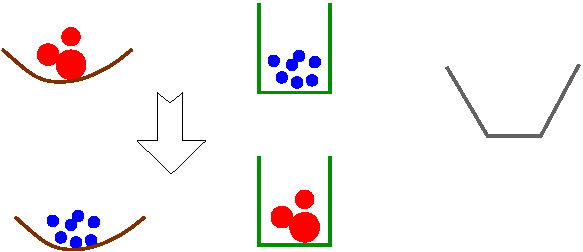
\includegraphics{Einterv_1.pdf}
 \caption{Intervertir les contenus de deux récipients}
 \label{fig:Einterv_1}
\end{figure}

Imaginons que l'on dispose de deux récipients contenant des objets. On veut les échanger. On sent bien qu'un troisième récipient est nécessaire et qu'il est alors facile de l'utiliser transitoirement.(Figure \ref{fig:Einterv_1})\newline
Dans la vraie vie, un récipient se \emph{vide} dans un autre ce qui n'est pas le cas avec des noms et des assignations. On pourrait imaginer que le récipient ne se vide pas mais que son contenu se duplique, ce n'est pas le cas non plus.

Considérons le code Python suivant
\begin{verbatim}
# initialisation
nom1 = "MickeydeTravers"
nom2 = "PetitsRondsBleus"
#Echange
nom3 = nom1
nom1 = nom2
nom2 = nom3
#Verification
print(nom1)
print(nom2)
\end{verbatim}
Après l'exécution de la première ligne du code ci dessus, quel est le type de l'objet désigné par \texttt{nom1}?
Quelle commande supplémentaire peut-on faire exécuter pour s'assurer qu'une assignation "ne vide pas" le nom placée à droite ?
Expliquez pourquoi le code suivant prouve que l'assignation ne copie pas les valeurs.
\begin{verbatim}
# initialisation
nom1 = ["disqueRouge1","disqueRouge2","disqueRouge3"]
nom2 = "PetitsRondsBleus"
print("valeurs initiales")
print(nom1)
print(nom2)

#Echange
nom3 = nom1
nom1 = nom2
nom2 = nom3

#Verification
print("échange")
print(nom1)
print(nom2)

print("modification")
print(nom3)
nom3.remove("disqueRouge2")
print(nom3)
print(nom2)
\end{verbatim}
Après l'exécution de la première ligne du code ci dessus, l'objet désigné par \texttt{nom1} est d'un type cité dans la partie 1. Principes; quel est ce type? Une propriété de ce type explique les résultats de l'exécution de ce code; laquelle? \newline
En utilisant une terminologie venant d'autres langages, on peut dire que l'assignation en Python se fait toujours \emph{par référence} et non \emph{par valeur}. C'est la raison fondamentale pour laquelle l'utilisation du mot \emph{nom} est préférable à celle de \emph{variable}.
